%======================================================================
\chapter{Background}
%======================================================================

\section{Hollow-Core Photonic Crystal Fiber}
\subsection{Conventional TIR Guidance}

\subsection{Bragg Gratings}
\begin{figure}[h!]
	\centering
	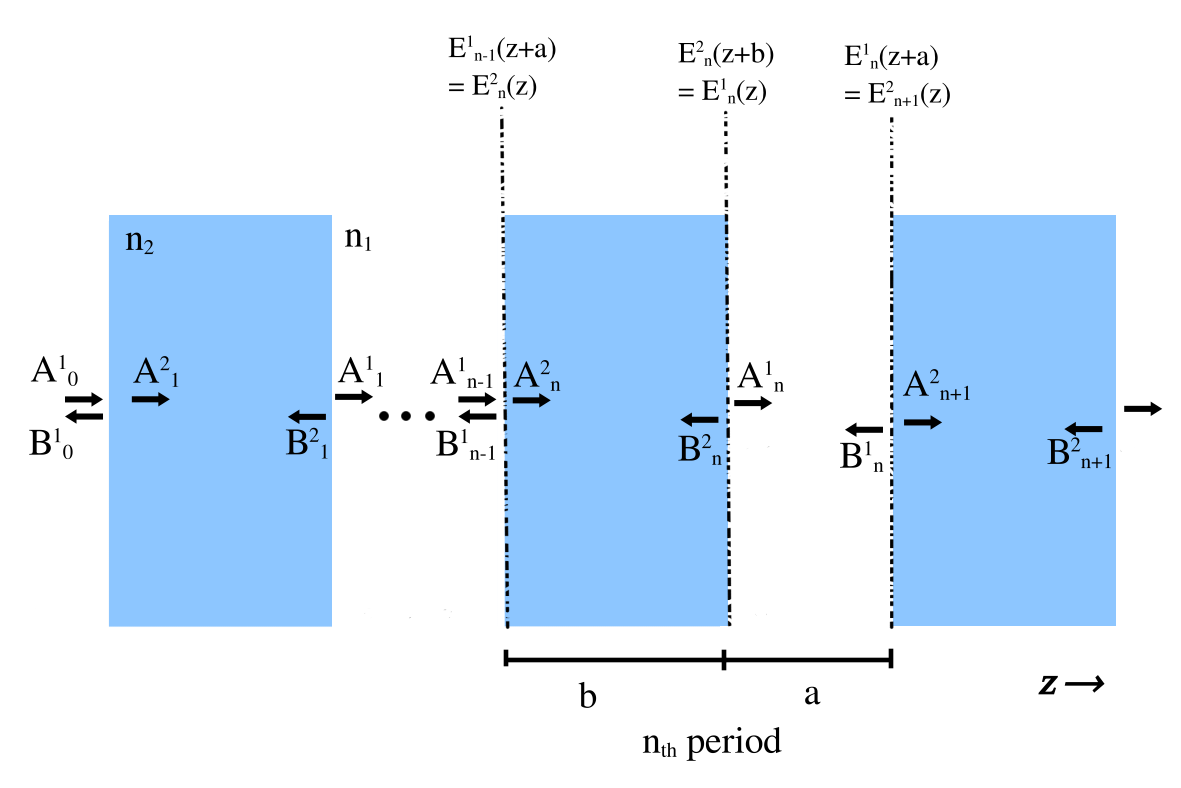
\includegraphics[width=\textwidth]{./Figures/HCPCF/DBR.png}
	\caption{Schematic of quarter wavelength stack}
\end{figure}
\clearpage
\begin{equation}
	\begin{aligned}
		E^1_n(z) &= A^1_n e^{-ik_{z1}(z-(n-1)a)} + B^1_n e^{ik_{z1}(z-(n-1)a)};  (n-1)a+b<z<na\\
		E^2_n(z) &= A^2_n e^{-ik_{z2}(z-(n-1)a)} + B^2_n e^{ik_{z2}(z-(n-1)a)};  (n-1)a<z<(n-1)a+b\\
	\end{aligned}
\end{equation}
Where $k _j= \frac{2\pi}{n_j}$
The boundary conditions:\\
continuous between the layers:
\begin{equation}
		E^1_n(z) = E^2_n(z+b)
\end{equation}
The second condition is that the electric field is smooth, which can be established in the perpendicular magnetic field. Assuming that the electric field is linearly polarized $E(z) = \boldsymbol{\hat{x}}E(z)$, then the magnetic field (via Faraday's law) $H(z) = \boldsymbol{\hat{y}}H(z)$.

\begin{equation}
	\begin{aligned}
		H^1_n(z) &=\frac{1}{\eta_1}[A^1_n e^{-ik_{z1}(z-(n-1)a)} - B^1_n e^{ik_{z1}(z-(n-1)a)}]\\
		H^2_n(z) &= \frac{1}{\eta_2}[A^2_n e^{-ik_{z2}(z-(n-1)a)} - B^2_n e^{ik_{z2}(z-(n-1)a)}]
	\end{aligned}
\end{equation}

\begin{equation}
	\begin{aligned}
			A^2_n(z) = \frac{1}{2}[E^2_n(z) + \eta_2 H^2_n(z)]\\
			B^2_n(z) = \frac{1}{2}[E^2_n(z) - \eta_2 H^2_n(z)]
	\end{aligned}
\end{equation}
Where the impedance $\eta_2 = \frac{\eta_0}{n2}$ \\
Putting these relations into a matrix form we can find a a solution for the transition boundary:
\begin{equation*}
	\begin{aligned}
		\begin{bmatrix}E^1_{n-1}(z+a)\\H^1_{n-1}(z+a) \end{bmatrix} 
		&= \begin{bmatrix}E^2_n(z)\\H^2_n(z) \end{bmatrix}\\
		 \begin{bmatrix}1 & 1\\\eta_1^{-1} & -\eta_1^{-1}\end{bmatrix}\begin{bmatrix}A^1_{n-1}(z+a)\\B^1_{n-1}(z+a) \end{bmatrix}
		 &=\begin{bmatrix}1 & 1\\\eta_2^{-1} & -\eta_2^{-1}\end{bmatrix}\begin{bmatrix}A^2_n(z)\\B^2_n(z) \end{bmatrix} \\
		\begin{bmatrix}A^1_{n-1}(z+a)\\B^1_{n-1}(z+a) \end{bmatrix}
		&= M_{1\rightarrow2}\begin{bmatrix}A^2_n(z)\\B^2_n(z) \end{bmatrix}\\
	\end{aligned}
\end{equation*}

\begin{equation}
	\begin{bmatrix}A^1_{n-1}(z+a)\\B^1_{n-1}(z+a) \end{bmatrix}
	= M_{1\rightarrow2}\begin{bmatrix}A^2_n(z)\\B^2_n(z) \end{bmatrix}\\
\end{equation}

The transition matrix:
\begin{equation}
	M_{1\rightarrow2} = 
	\frac{1}{2}\begin{bmatrix}1+\frac{k_2}{k_1} & 1-\frac{k_2}{k_1}\\1-\frac{k_2}{k_1} & 1+\frac{k_2}{k_1}\end{bmatrix}
\end{equation}

The plane wave propagating though the material will acquire a phase:  
\begin{equation}
	M_{n_2} = \begin{bmatrix}e^{ik_{z2}b} & 0\\0 & e^{-ik_{z2}b}\end{bmatrix}\\
\end{equation}

Thus the travel through the n2 material can be summarized by
\begin{equation}
	\begin{aligned}
		\begin{bmatrix}A^1_{n-1}(z+a)\\B^1_{n-1}(z+a) \end{bmatrix}
		M_{1\rightarrow2}M_{n2}
		\begin{bmatrix}A^2_n(z+b)\\B^2_n(z+b) \end{bmatrix}
	\end{aligned}
\end{equation}

For the electric field through the n1 region :
\begin{equation}
	M_{1\rightarrow2} = 
	\frac{1}{2}\begin{bmatrix}
		1+\frac{k_1}{k_2} & 1-\frac{k_1}{k_2}\\
		1-\frac{k_1}{k_2} & 1+\frac{k_1}{k_2}
	\end{bmatrix}
	\begin{aligned}
		&M_{n_1} =
		\begin{bmatrix}
			e^{ik_{z1}a} & 0\\
			0 & e^{-ik_{z1}a}
		\end{bmatrix}\\
	\end{aligned}
\end{equation}

Becomes one periodic transition matrix:
\begin{equation*}
	M_p = M_{1\rightarrow2}M_{n2}M_{2\rightarrow1}M_{n1} = \begin{bmatrix}m_{11} & m_{12}\\m_{21} & m_{22}\end{bmatrix}\\ 	
\end{equation*}

For an N period block:
\begin{equation*}
	\begin{aligned}
		\begin{bmatrix}A_0\\B_0 \end{bmatrix} 
		&=\frac{1}{2}\begin{bmatrix}1 & \eta_1\\1 & -\eta_1\end{bmatrix} 
		(M_p)^N 
		\begin{bmatrix}1 & \eta_1\\1 & -\eta_1\end{bmatrix}\begin{bmatrix}A_{(N+1)}\\0\end{bmatrix}\\
		\begin{bmatrix}1 \\\eta_1^{-1}\end{bmatrix}A_{(N+1)}
		&= \begin{bmatrix}(-\frac{\eta_2}{\eta_1})^N+(-\frac{\eta_1}{\eta_2})^N \\ (-\frac{\eta_2}{\eta_1})^N-(-\frac{\eta_1}{\eta_2})^N\end{bmatrix}A_{(N+1)}\\
		R &= \Bigg|\frac{(-\frac{\eta_2}{\eta_1})^N-(-\frac{\eta_1}{\eta_2})^N}{(-\frac{\eta_2}{\eta_1})^N+(-\frac{\eta_1}{\eta_2})^N}\Bigg|^2\\
		&=\Bigg|\frac{1-(\frac{\eta_1}{\eta_2})^{2N}}{1+(\frac{\eta_1}{\eta_2})^{2N}}\Bigg|^2; \eta_i = \frac{\eta_0}{\eta_i}, i = 1, 2
	\end{aligned}
\end{equation*}

\subsection{Band Structure}

\subsection{Photonic Crystal Bandgap}


\subsection{Bandgap Shift}
\begin{equation}
	\lambda = \lambda_0\sqrt{\frac{1-N^{-2}}{1-N_0^{-2}}}
\end{equation}

\begin{equation}
N_0 = \frac{n_{air}}{n_{glass}}, N = N_0 = \frac{n_{liquid}}{n_{glass}} 
\end{equation}
$n_{air} < n_{glass} < n_{liquid}$


\subsection{Mode Distribution}

a) For a two-level atom, the coupling constant -- g -- [Eq. 2.6] scales inversely to this 'effective mode area'  [Eq. before 2.1]  (in the interaction energy term between atom and the field). Ref: https://journals.aps.org/pra/abstract/10.1103/PhysRevA.65.033832
(A single photon interacts more strongly when the mode is more confined. And, if the mode is like a Gaussian [given by the mode function f(x,y) ] the photon interacts more strongly if the atom is placed in the center of the mode.)
b) Apparently, this coupling constant term tells us parameters such as:
 i) how likely it is for an excitation in the emitter is released into the waveguide mode $(\gamma_{1D}), versus free-space (\gamma_0). [Eq. 2.10]. $
 
  ii) optical depth (OD) for a single atom is (about) the ratio of $ (\gamma_{1D})/ (\gamma_{0})$ or the ratio of the cross-section area of the atom to that of the effective mode-area. [Eq. 6 in Ref: Optical Nanofibers: a new platform for quantum optics: https://arxiv.org/pdf/1703.10533.pdf 
  or Pages: 39 - 40 of the PhD Thesis: M. Manzoni, New Systems for Quantum Nonlinear Optics https://upcommons.upc.edu/bitstream/handle/2117/114004/TMTM1de1.pdf?sequence=1\&isAllowed=y]
  
c) Optical depth (OD) tells about how opaque the system is. Transmitted intensity goes by $exp(-OD)$. Normally, N emitters might scale linearly to give an optical depth ~$N*OD$. But now (due to its position) each emitter might have its own mode area.

Examples of taking this into account (with maybe slightly different conventions) for atoms are mentioned in these two references: [ Section B. in Ref: https://journals.aps.org/pra/abstract/10.1103/PhysRevA.83.063830 and Appendix A. in https://journals.aps.org/prapplied/abstract/10.1103/PhysRevApplied.10.044034]


